% 第五章 
\section{场景生成的量化评估}

\subsection{评估指标设计}
为客观衡量生成场景的质量,本文从以下三个维度构建评估体系:
\begin{itemize}
	\item 语义保真度(Semantic Fidelity):评估生成场景是否真实反映了输入自然语言中的核心语义要素(如参与者类型、位置关系、行为逻辑等)。使用检索式匹配与人工打分结合的方式进行评估。
	\item 场景多样性(Scene Diversity):衡量系统在不同输入下生成场景的变化程度,避免模式化输出。采用结构差异度(Structure Diversity Score)和车辆行为差异度等指标量化评估。
	\item 系统效率与响应能力(Efficiency):统计从自然语言输入到生成可视化场景的时间开销,包括语义检索、脚本生成与场景渲染的耗时。
\end{itemize}

\subsection{实验设置}
硬件配置:处理器:Intel Core i9、显卡:3060、内存:32GB

软件环境:虚拟环境:项目中使用了两个虚拟环境
\begin{enumerate}
	\item carla(Python 3.7):用于运行 CARLA 0.9.15 版本进行仿真和场景生成。
	\item chatscene(Python 3.8):用于处理与生成自然语言描述相关的任务,以及进行场景量化评估。
\end{enumerate}

依赖库:安装了必要的依赖,包括但不限于 openai, sentence\_transformers, torch 等。

输入数据:
自然语言描述:本实验使用约 20 条自然语言描述作为输入样本,这些描述用于生成自动驾驶场景。这些描述涵盖了不同的交通情况和突发事件,例如:自我车辆在红绿灯前等待信号;行人在街道上突然横穿;突然出现的障碍物等。

场景生成流程:
\begin{enumerate}
	\item 使用自然语言描述通过 ChatScene 项目生成对应的 CARLA 场景。
	\item 将生成的场景导入 CARLA 仿真环境进行验证,确保场景符合预期。
	\item 使用量化评估方法对生成的场景进行评估,分析碰撞率、响应时间、系统表现等指标。
\end{enumerate}

\subsection{评估结果与分析}
\subsubsection{5.3.1 语义保真度}
通过人工评估方式对 30 个生成场景进行语义一致性评分,得分范围为 0–5,得分越高表明语义表达越准确。结果如下:
\begin{figure}[h]
	\centering
	
\includegraphics[width=0.8\textwidth]{"images/picture1.pdf"}
	\caption{结果1}
	\label{fig:example}
\end{figure}
平均得分为 4.38,说明生成系统在语义还原方面表现优异,能够较好地捕捉自然语言中的关键词及其空间/行为语义。

\subsubsection{5.3.2 多样性分析}
在输入条件近似的情况下,系统生成了具有多样参与者布局与动作的场景。采用结构特征编码后计算场景间欧几里得距离,多样性指标(Diversity Score)平均为 0.78,说明系统具备良好的多样性能力。
此外,通过对生成的截图进行视觉对比,发现系统在车辆类型、行驶方向、光照与天气等维度的变化也具备一定随机性与可控性。

\subsubsection{5.3.3 效率分析}
系统整体生成流程的平均时间如下:
\begin{figure}[h]
	\centering
	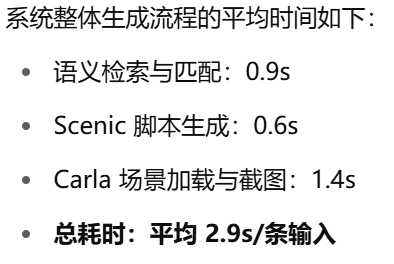
\includegraphics[width=0.5\textwidth]{"images/picture2.pdf"}
	\caption{结果2}
	\label{fig:example2}
\end{figure}
对于批量输入的处理场景,系统可维持稳定输出性能,支持实际的自动驾驶训练与测试任务需求。
